\documentclass[a4paper, 11pt, oneside]{article}

\newcommand{\plogo}{\fbox{$\mathcal{PL}$}} 
\usepackage{amsmath}
\usepackage{stix}
\usepackage{amsthm}
\usepackage[utf8]{inputenc} 
\usepackage[T1]{fontenc} 
\usepackage{fancyhdr}
\pagestyle{fancy}
\usepackage{enumitem}
\usepackage{graphicx}
\usepackage{graphicx}
\usepackage{amssymb}
\usepackage{supertabular}
\usepackage[spanish]{babel}
\usepackage{hyperref}
\usepackage{verse}
\usepackage{biblatex}
\begin{document} 

\begin{titlepage} 

	\centering 
	
	\scshape 
	
	\vspace*{\baselineskip} 
	
	
	
	\rule{\textwidth}{1.6pt}\vspace*{-\baselineskip}\vspace*{2pt} 
	\rule{\textwidth}{0.4pt} 
	
	\vspace{0.75\baselineskip} 
	
	{\LARGE Análisis de Poemas con Glove y SOM}	
	\vspace{0.75\baselineskip} 
	
	\rule{\textwidth}{0.4pt}\vspace*{-\baselineskip}\vspace{3.2pt}
	\rule{\textwidth}{1.6pt} 
	
	\vspace{2\baselineskip} 
	

	Redes Neuronales
	
	\vspace*{3\baselineskip} 
	
	
	
	Alumna:
	
	\vspace{0.5\baselineskip} 
	
	{\scshape\Large Karla Adriana Esquivel Guzmán}
	\vspace{0.5\baselineskip} 
	\vfill
	
\includegraphics[scale=0.65]{unam.jpg}
	
	\textit{UNIVERSIDAD NACIONAL AUTONOMA DE MEXICO} 
	
	\vfill
	
	
	
	
	\vspace{0.3\baselineskip} 
	
    15/Junio/2020
	
	 

\end{titlepage}
\newpage
\section*{Introducción}

En este proyecto se buscará la forma de clasificar poemas de diversos autores/poetas, a partir de la vectorización de cada uno de sus poemas, esto lo lograremos con ayuda de Glove, la representación vectorial de cada poema servirá para alimentar a SOM que al final nos dará como resultado una malla con los resultados de dicha clasificación.

\section*{Objetivo}
¿Cómo vamos a vectorizar los poemas y obtener su clasificación?
\section*{Métodos}
Principalmente se va a utilizar Glove,6b pero \textbf{¿Qué es Glove?} Glove es un modelo que utiliza un algoritmo de \textbf{aprendizaje no supervisado} que sirve para obtener la representación vectorial de palabras, esto se logra mapeando las palabras en un espacio dónde la distancia esta relacionada con respecto a su similitud semántica. El aprendizaje automatizado se basa en dar un conjunto de información sin etiquetas y a partir de ello una red neuronal extrae dicha información y a raíz de encontrar patrones etiqueta dicha información para posteriormente clasificarla.
\subsection*{¿Cómo se vectoriza un Poema?}
El proceso de vectorización de un poema conlleva varios pasos que a continuación voy a enunciar:
\begin{enumerate}
    \item Hay que tokenizar el poema, primero que nada debemos eliminar las palabras vacias o palabras sin significado (stop words), es decir palabras como artículos, peroposiciones, pronombres, etcétera, dichas palabras van a estar repetidas en muchos poemas, el dejarlas simplemente complicara más la diferenciación de los poemas. Como ejemplo tomaré el siguiente poema
    \poemtitle{The Appeal}
    \begin{verse}
        It I have given you delight\\ By aught that I have done,\\ Let me lie quiet in that night\\ Which shall be yours anon: \\And for the little, little, span\\The dead are born in mind,\\ Seek not to question other than\\ The books I leave behind.
    \end{verse}
    una vez eliminadas las palabras vacias obtendremos la siguiente lista:
    
    ['given', 'delight', 'aught', 'done', 'let', 'lie', 'quiet', 'night', 'shall', 'anon', 'little', 'little', 'span', 'dead', 'born', 'mind', 'seek', 'question', 'books', 'leave', 'behind']
\item Sin embargo como se puede notar aun tenemos palabras repetidas dentro de nuestra lista así que hay que eliminarlas, la lista final de palabras será la siguiente:

['anon', 'aught', 'behind', 'books', 'born', 'dead', 'delight','done', 'given', 'leave', 'let', 
'lie', 'little','mind', 'night', 'question', 'quiet', 'seek', 'shall', 'span']

\item Una vez que obtenemos la lista de palabras vamos a obtener el vector asociado a cada una de ellas utilizando Glove, para ejemplificar utilizaré la palabra books, la siguiente es su representación vectorial:
\begin{center}
    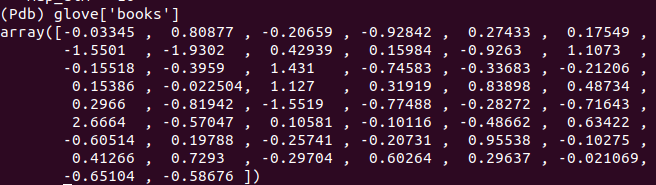
\includegraphics[scale=0.50]{Imagenes/booksglove.png}
\end{center}
\item Una vez obtenida la representación vectorial de cada una de las palabras, se debe obtener el promedio de los vectores, lo cual nos dará como resultado la representación vectorial del Poema, en este caso la representación del poema The Appeal es la siguiente:
\begin{center}
    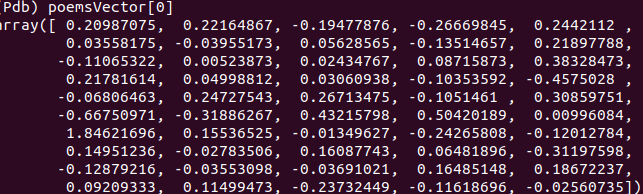
\includegraphics[scale=0.50]{Imagenes/poemvec.png}
\end{center}
\end{enumerate}
Si bien ya he mencionado los pasos a seguir para vectorizar un poema ahora queda hablar sobre la etapa de experimentación.
\subsection*{Experimentación}
Utilizando 60 poemas de 3 autores distintos, es decir en total 180 poemas, lo primero que hice fue vectorizar cada uno de estos poemas, posteriormente esta representación vectorial se la di como entrada a SOM, pero ahora surge otra pregunta \textbf{¿Qué es SOM?} SOM es un tipo de \textbf{Red Neuronal Autoasociativa} que utiliza aprendizaje no supervisado, representa vectores de dimensión alta a dimensión baja, en mi caso utilicé MiniSOM \url{https://pypi.org/project/MiniSom/} MiniSOM es una implementación de SOM. Ahora que ya mencioné esto voy a agregar el siguiente fragmento de código:
\begin{center}
    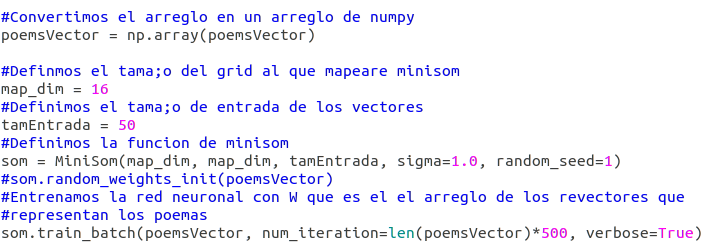
\includegraphics[scale=0.50]{Imagenes/SOM.png}
\end{center}
En el código anterior simplemente estamos configurando el tamaño de la entrada que en este caso son vectores de Glove de tamaño 50, la malla de tamaño $16 * 16$ y la semilla con la que va a ejecutarse y para el entrenamiento se define el número de iteraciones.
\section*{Resultados}
A continuación adjuntaré los resultados de diversos datos en los que me basé para la experimentación:
De experimentar con el conjunto de autores de una época similar:\\ 
1809-1849 Edgar Allan Poe(Amarillo),\\
1770-1850 William Wordsworth(Azul),\\
1757-1827 William Blake(Rojo)

\begin{center}
    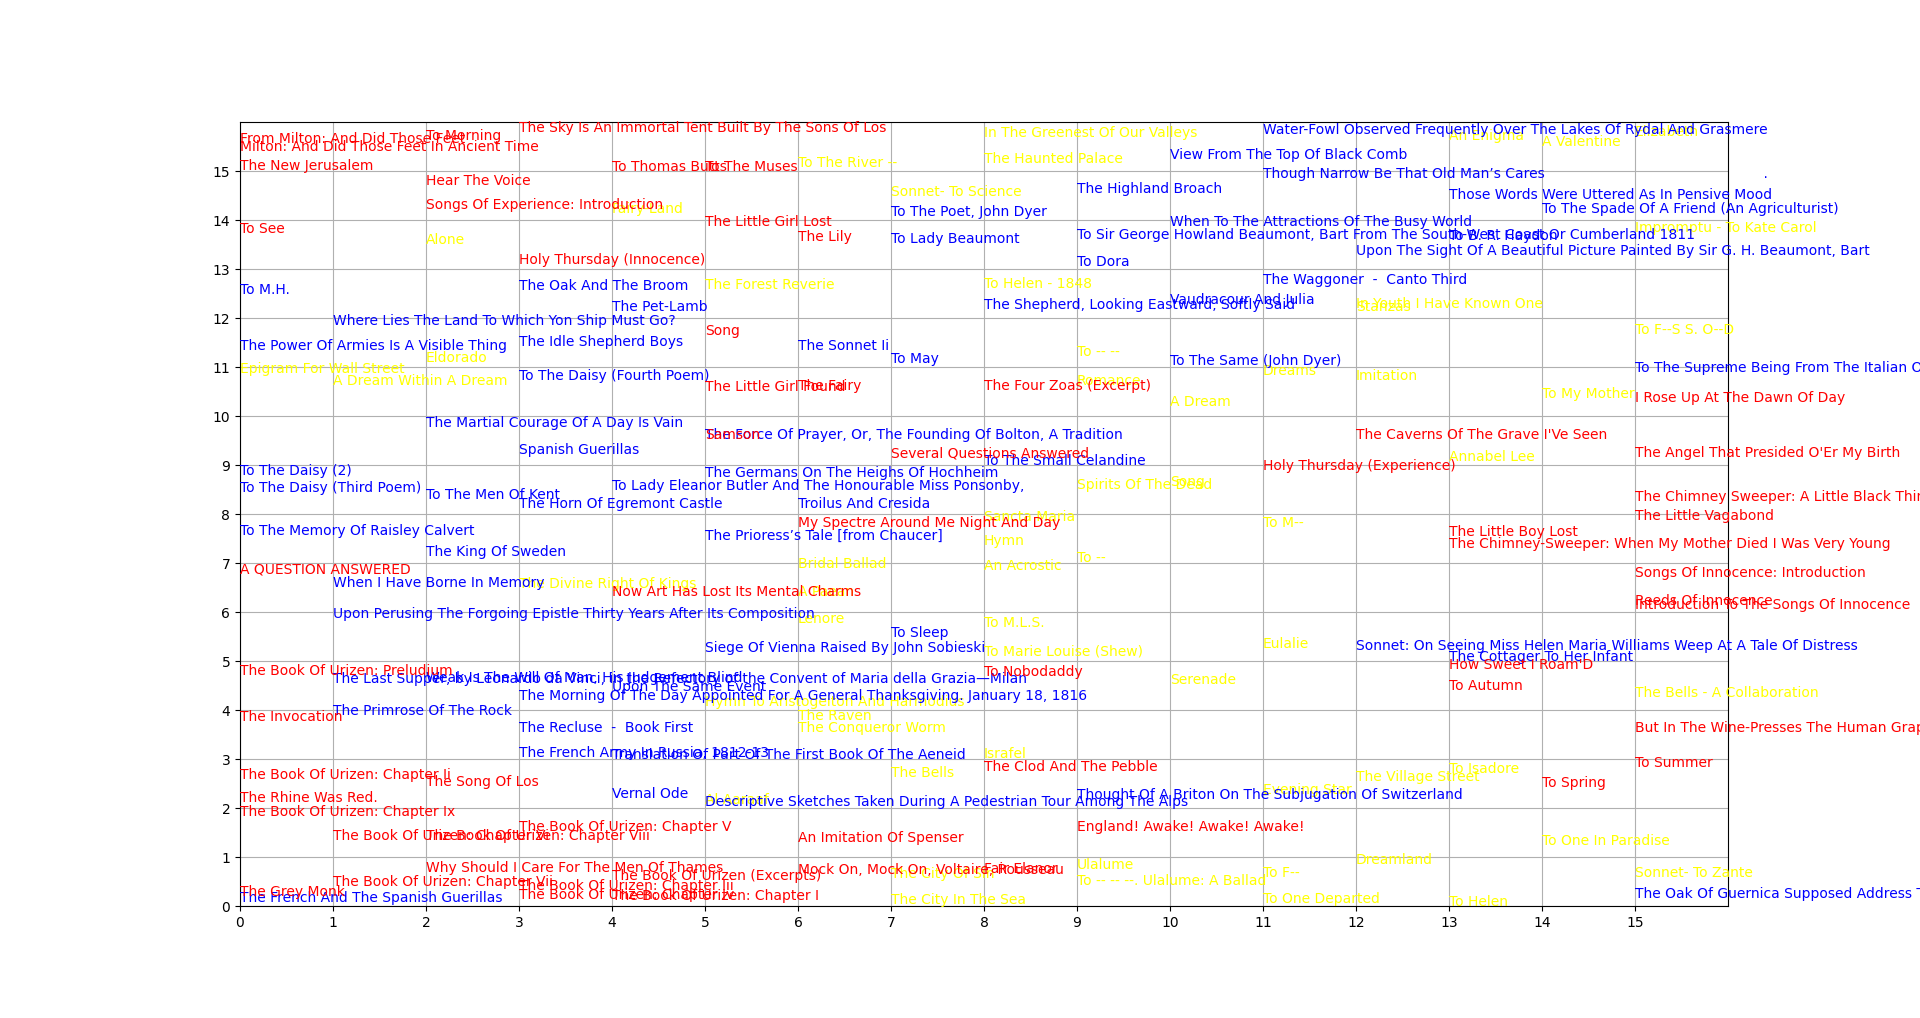
\includegraphics[scale=0.15]{Imagenes/1.png}
\end{center}
Conjunto de escritores de la misma nacionalidad en este caso Reino Unido\\
1608-1674 John Milton(Amarillo),\\
1770-1850 William Wordsworth(Azul),\\
1564-1616 William Shakespeare(Rojo),

\begin{center}
    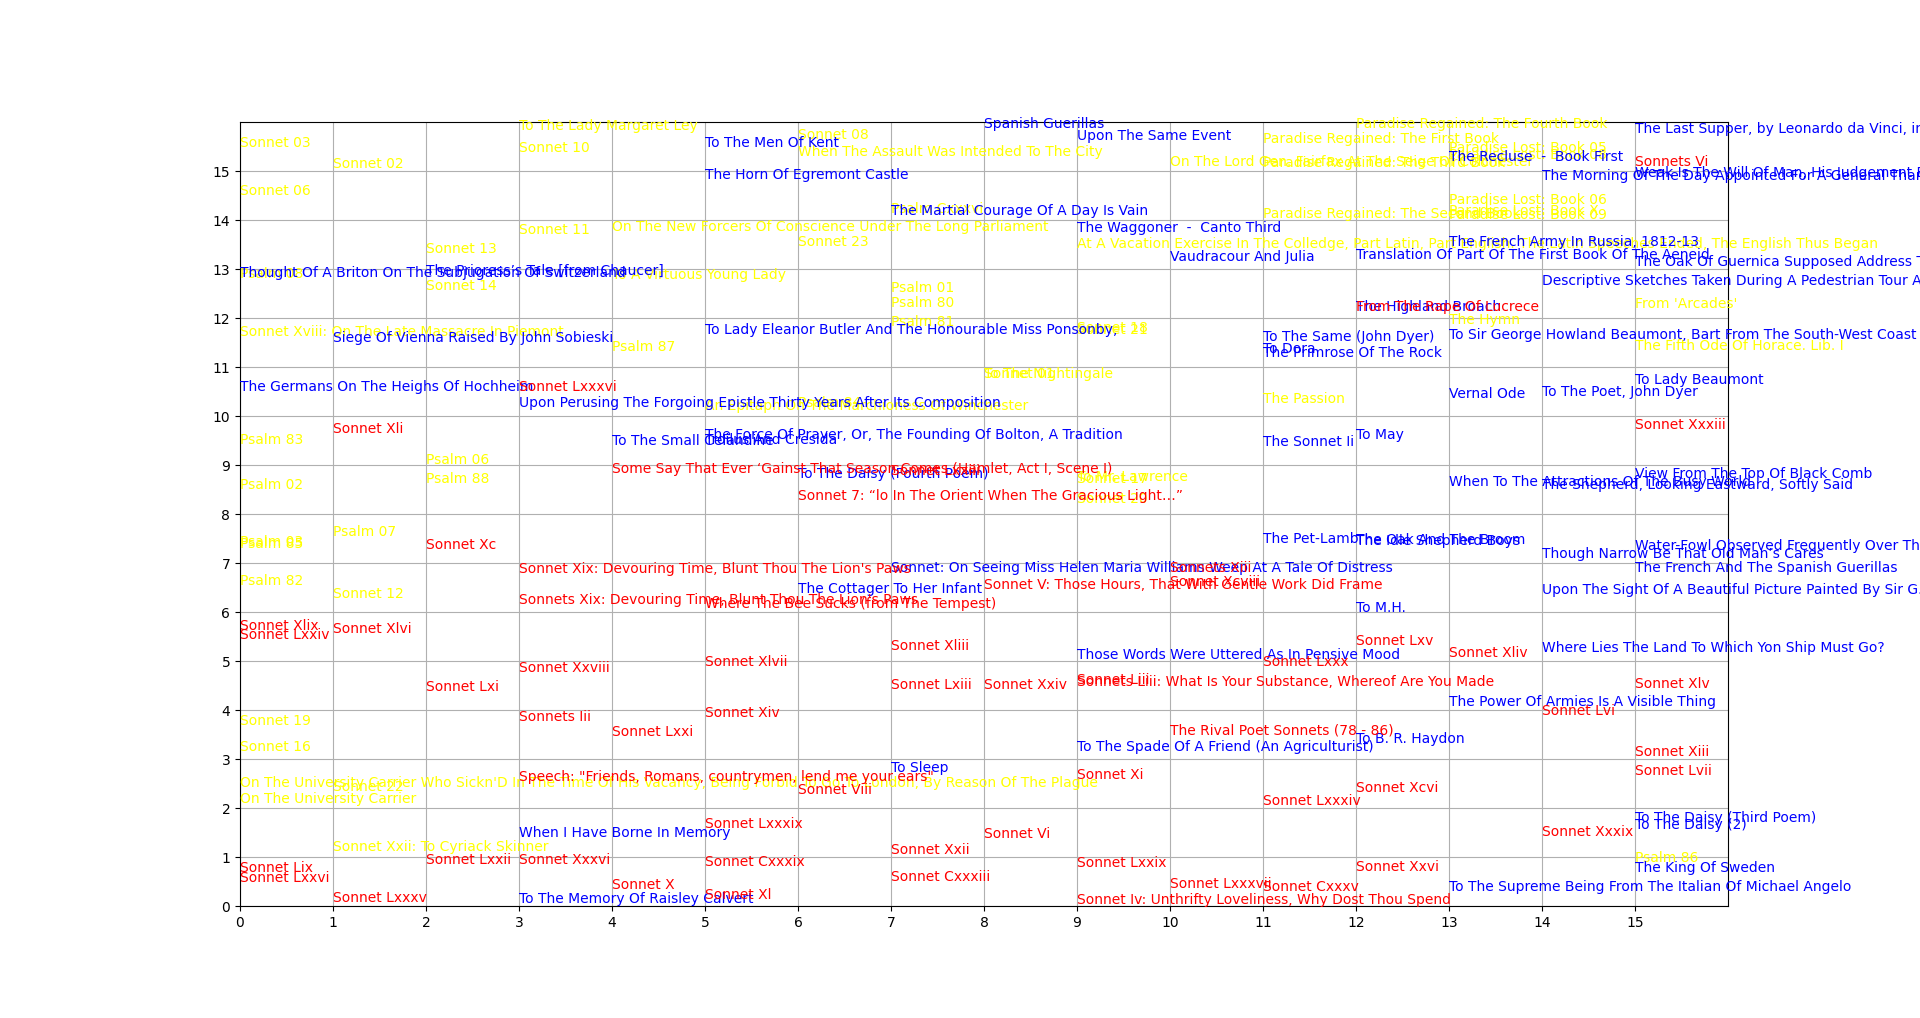
\includegraphics[scale=0.15]{Imagenes/2.png}
\end{center}
Conjunto de escritores del mismo país USA\\
1819-1892 Walt Whitman(Amarillo),\\
1809-1849 Edgar Allan Poe(Rojo),\\
1885-1972 Ezra Pound(Azul)
\begin{center}
    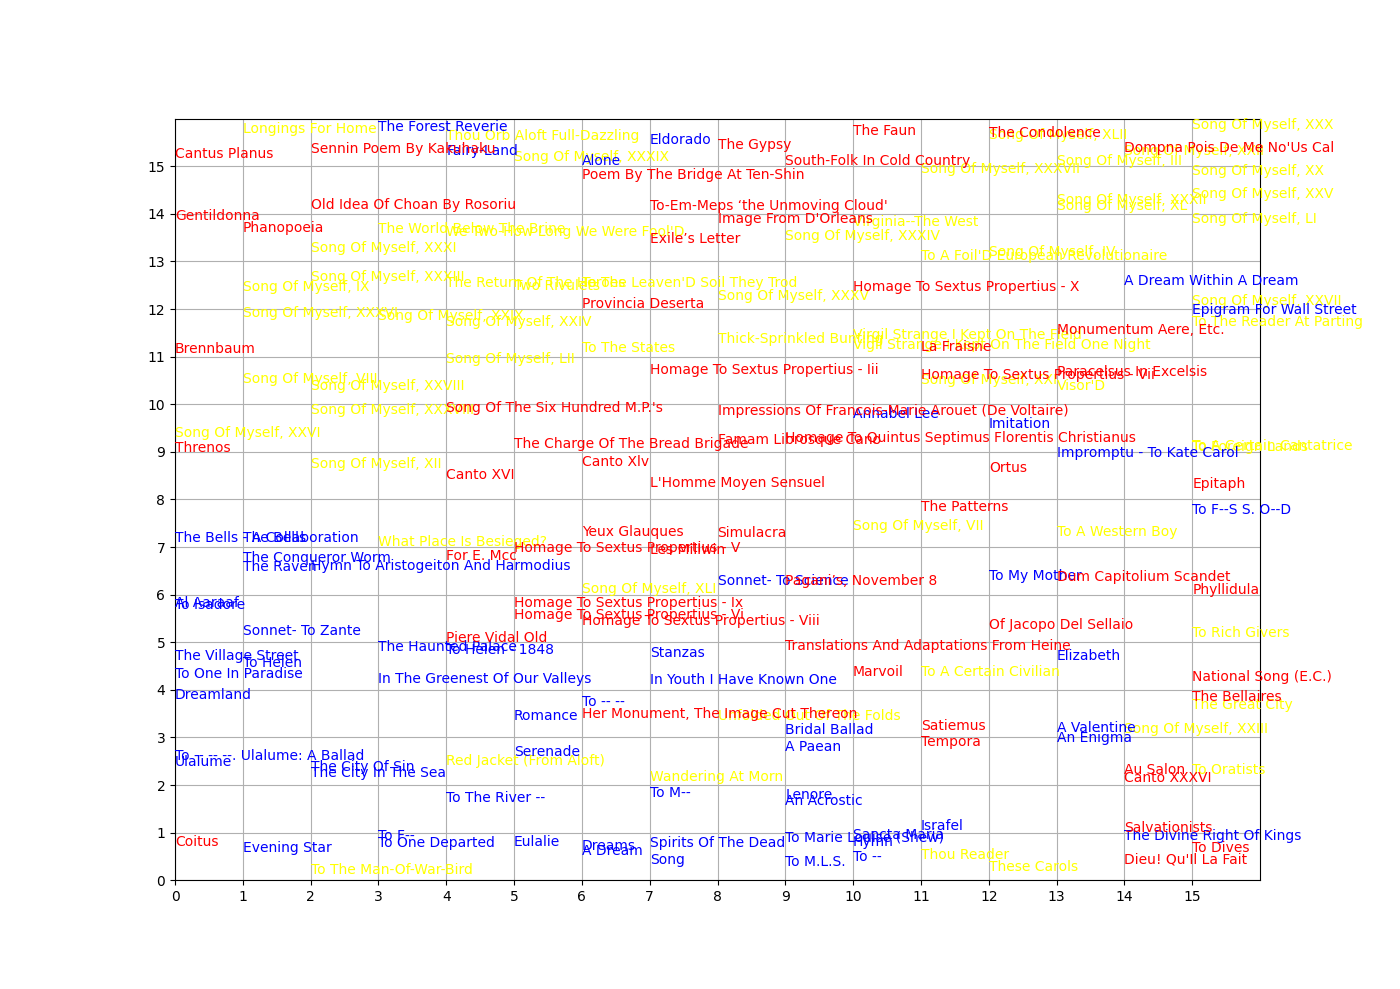
\includegraphics[scale=0.20]{Imagenes/3.png}
\end{center}
Conjunto de escritores diferentes épocas y diferetes nacionalidades\\
1564-1616 William Shakespeare(Amarillo), Reino Unido,\\
1865-1936 Rudyard Kipling(Azul), India,\\
1932-1963 Sylvia Plath(Rojo), Estados Unidos\\
Este primer resultado se obtuvo utilizando un vector de tamaño 50 con una malla de $16*16$
\begin{center}
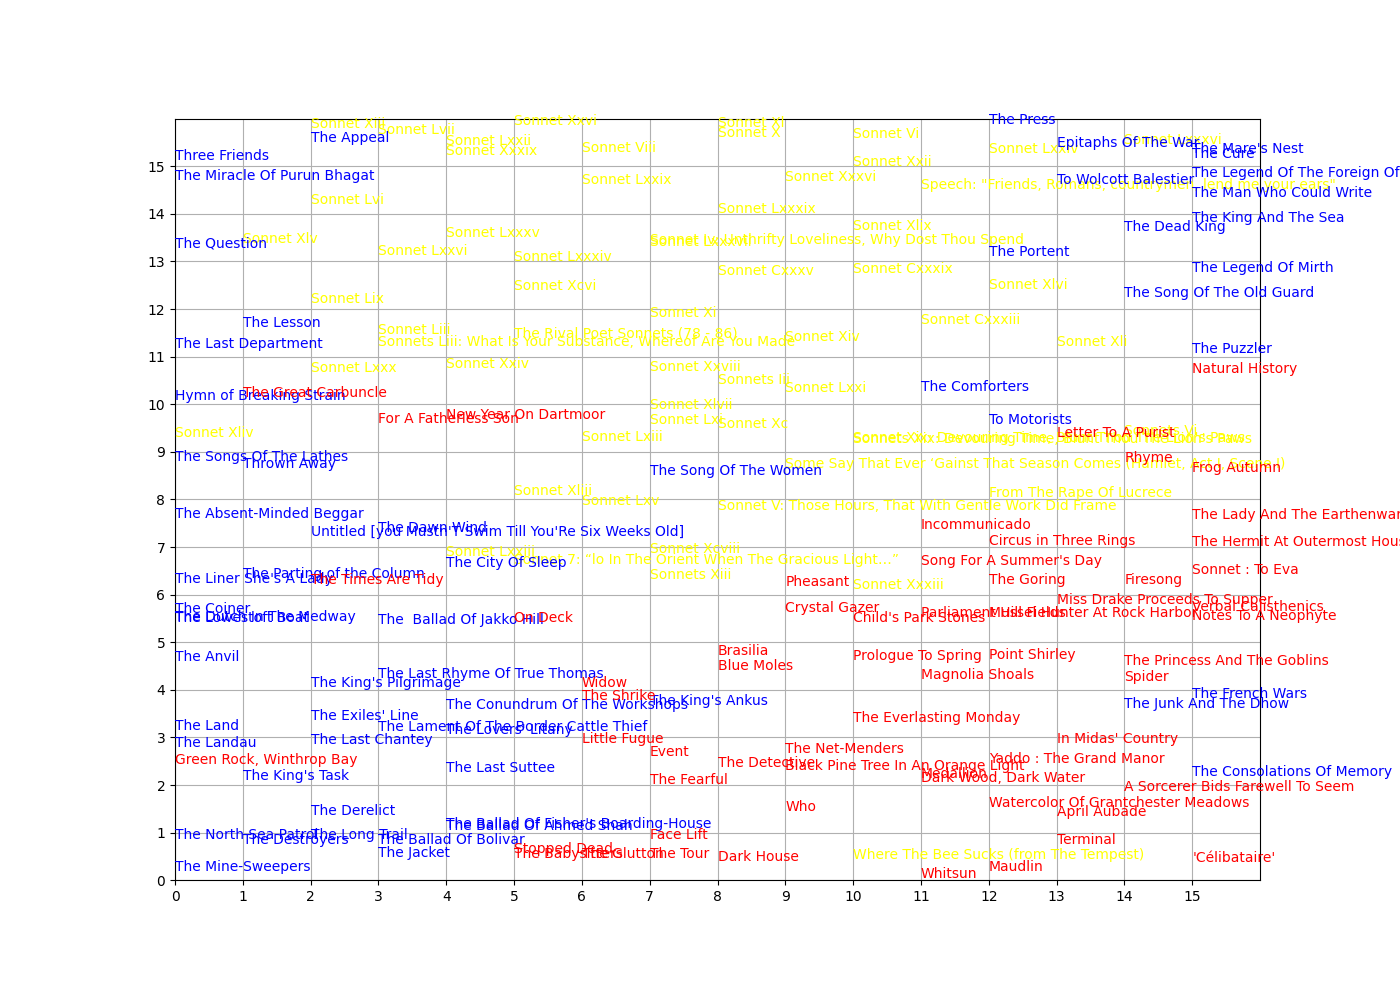
\includegraphics[scale=0.35]{Imagenes/WShakespeareRKiplingSPlathGlove50G16x16.png}    
\end{center}
Tamaño del vector: 50 malla: $40*40$
\begin{center}
    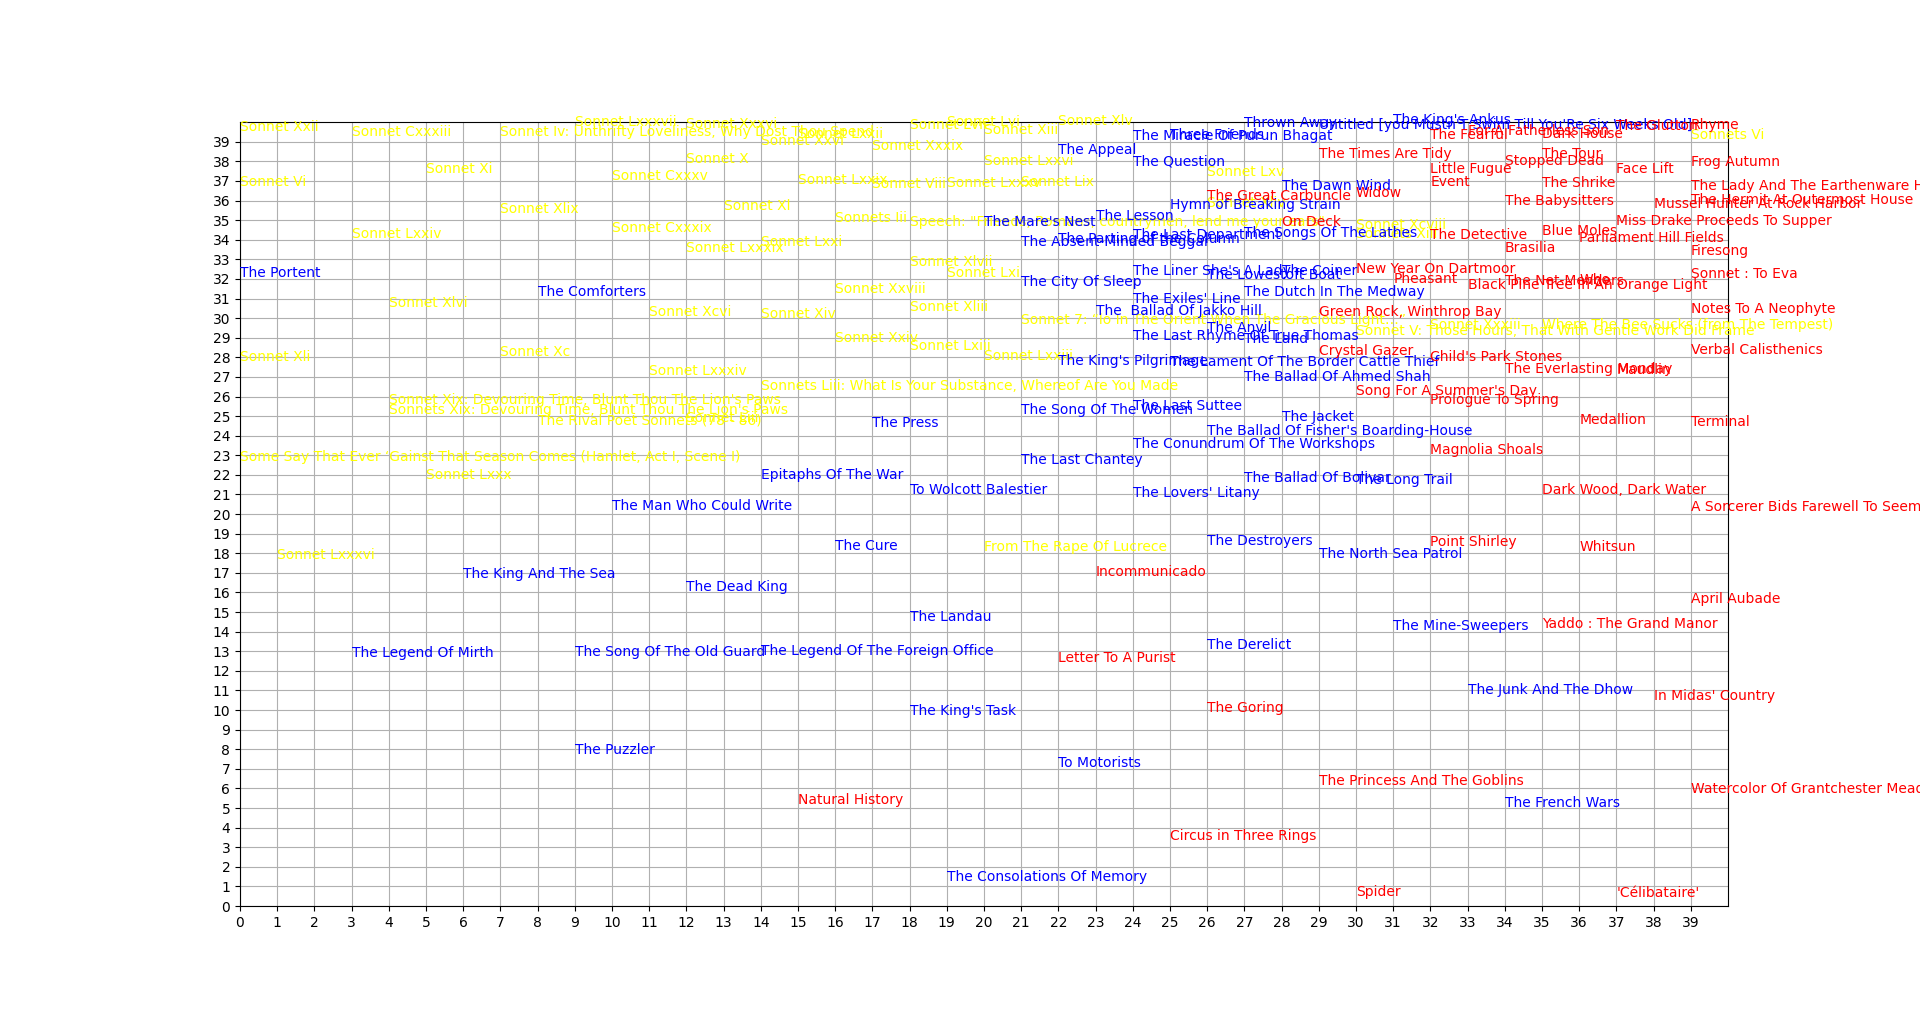
\includegraphics[scale=0.25]{Imagenes/WShakespeareRKiplingSPlathGlove50G40x40.png}
\end{center}
Tamaño del vector: 100 malla: $16*16$
\begin{center}
    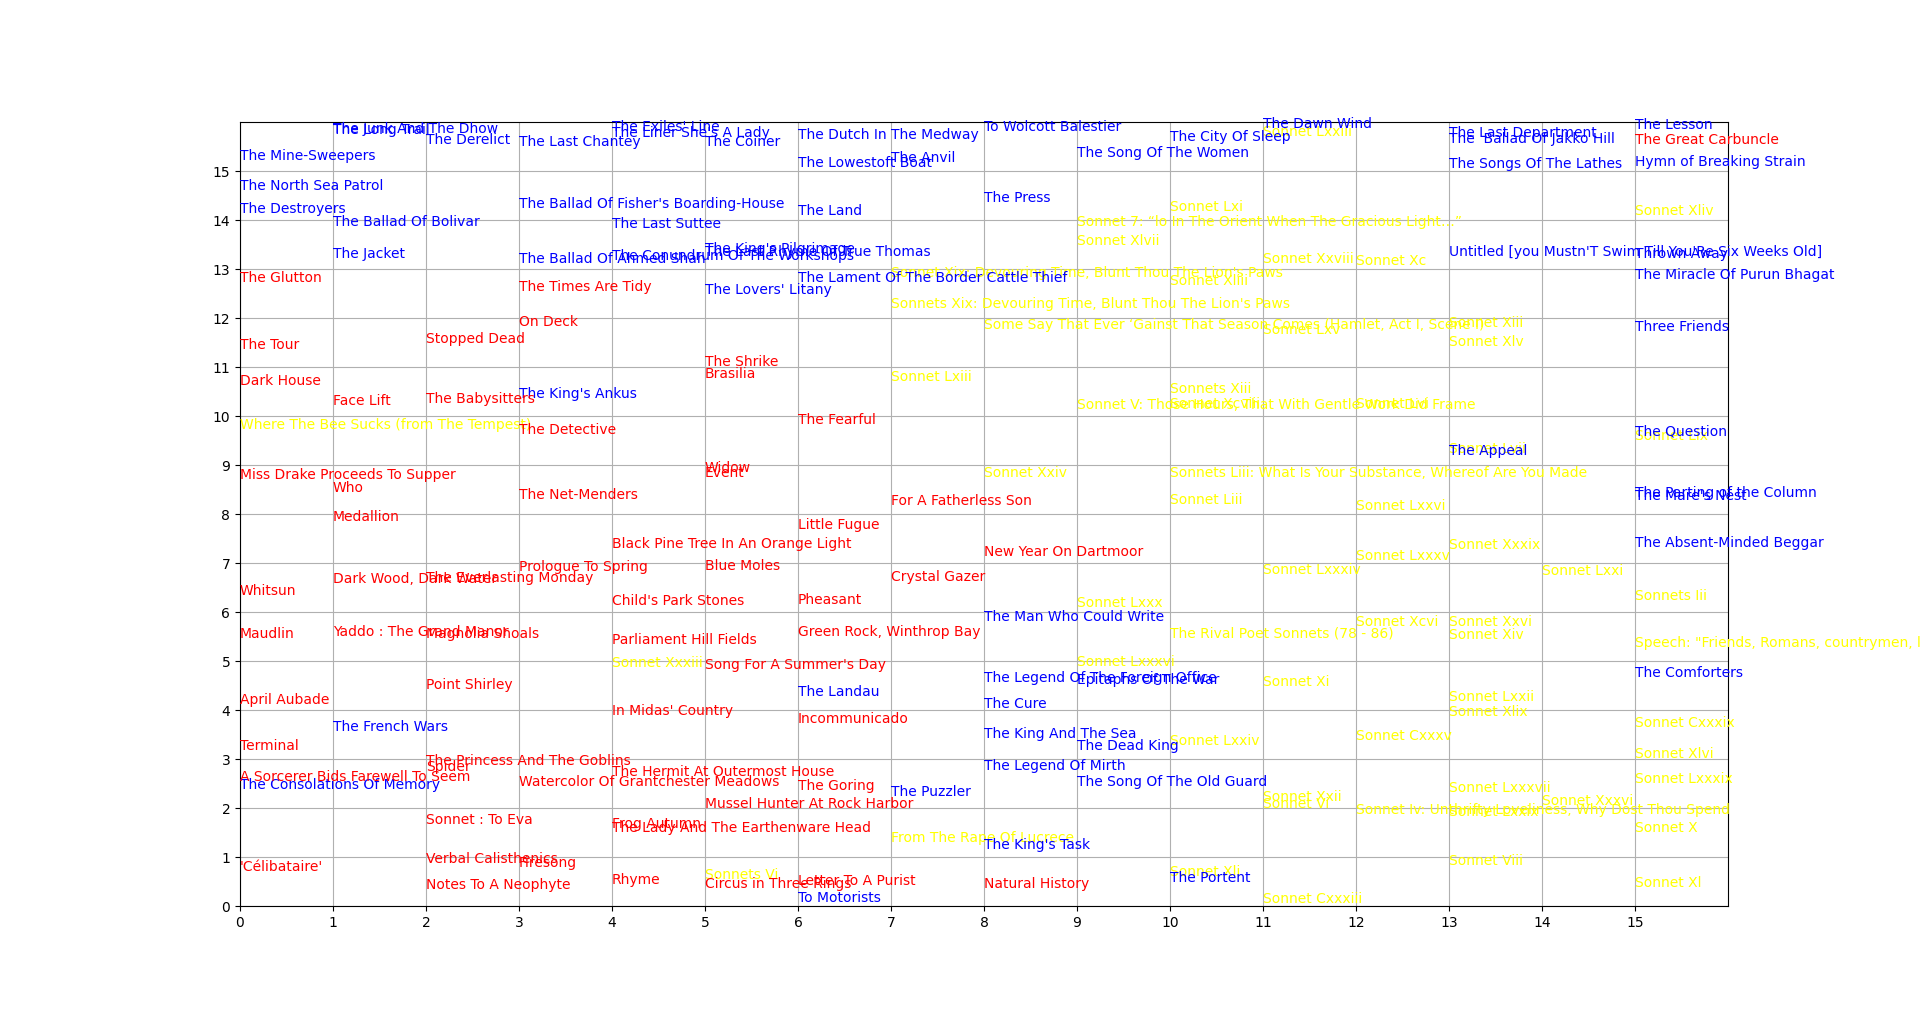
\includegraphics[scale=0.25]{Imagenes/WShakespeareRKiplingSPlathGlove100G16x16.png}
\end{center}
Tamaño del vector: 100 malla: $40*40$
\begin{center}
    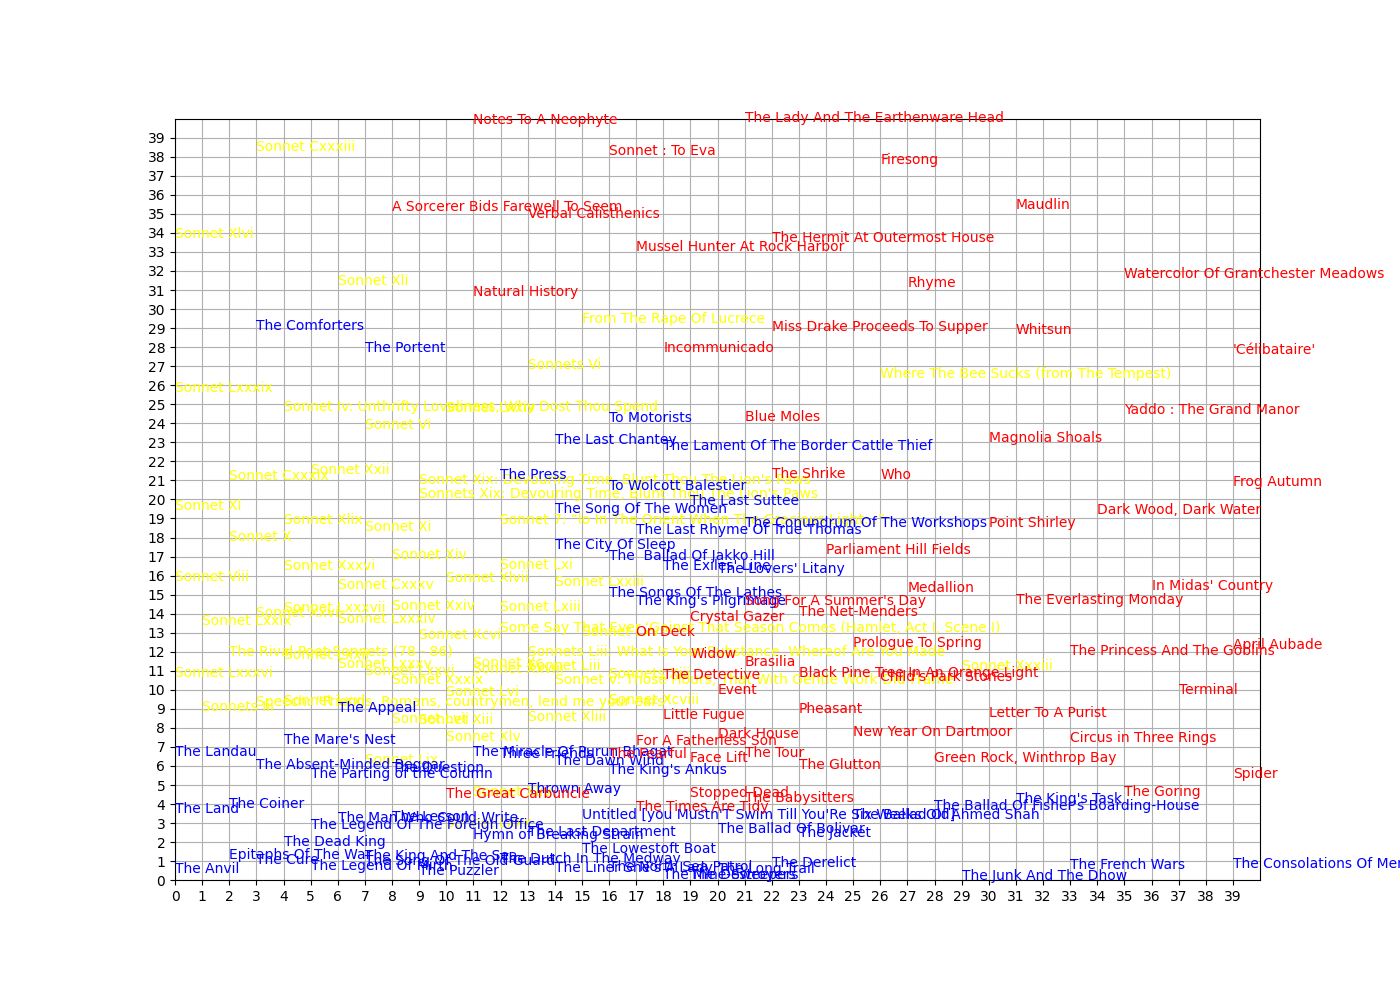
\includegraphics[scale=0.35]{Imagenes/WShakespeareRKiplingSPlathGlove100G40x40.png}
\end{center}
Tamaño del vector: 300 malla: $16*16$
\begin{center}
    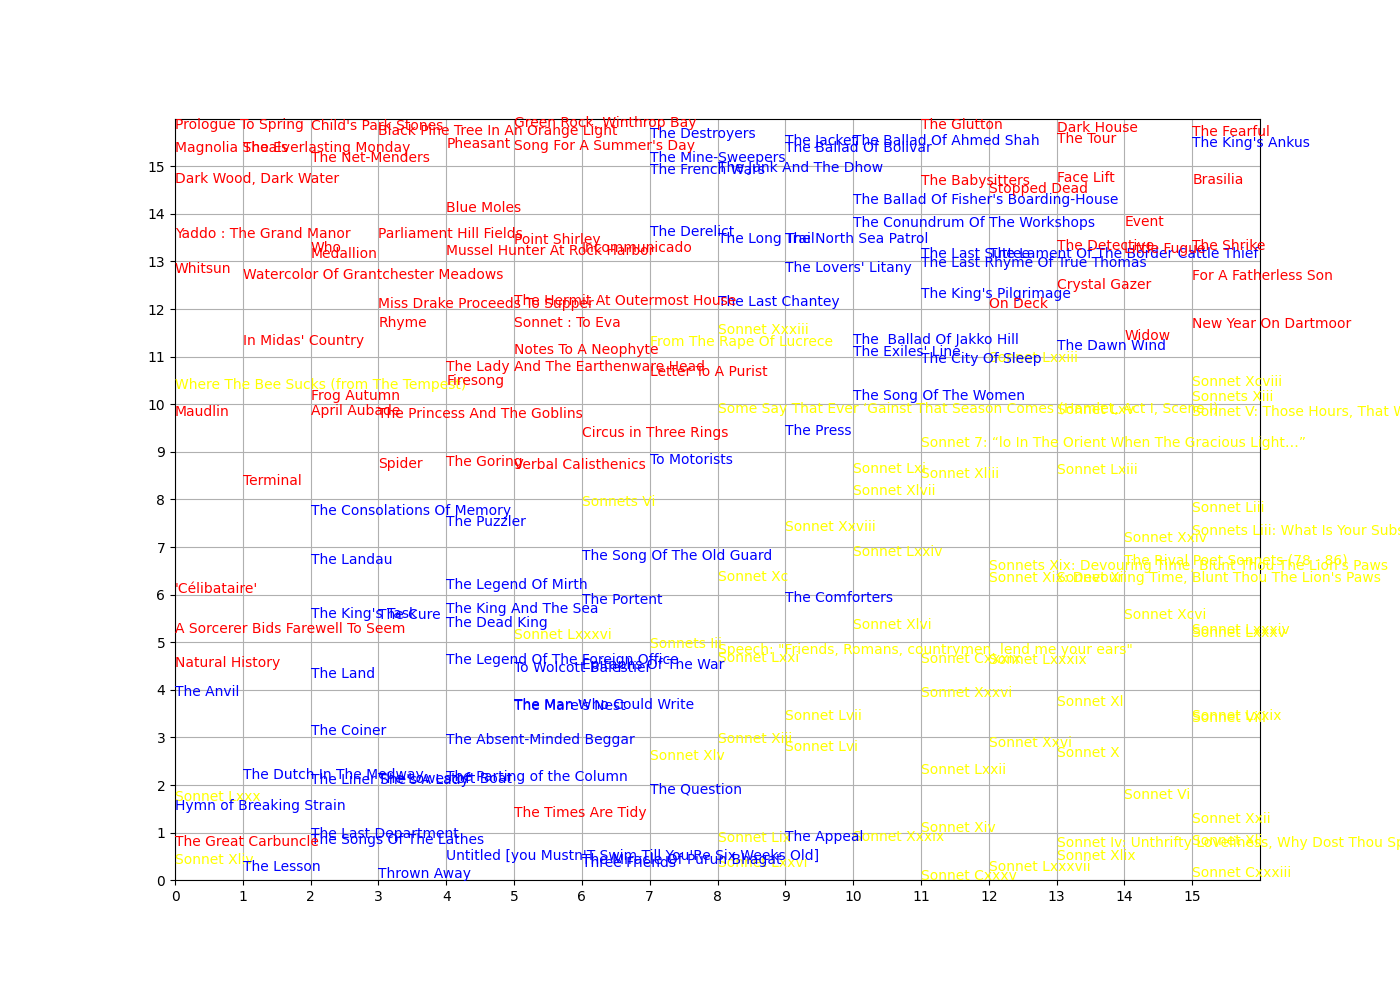
\includegraphics[scale=0.35]{Imagenes/WShakespeareRKiplingSPlathGlove300G16x16.png}
\end{center}
Tamaño del vector: 300 malla: $40*40$
\begin{center}
    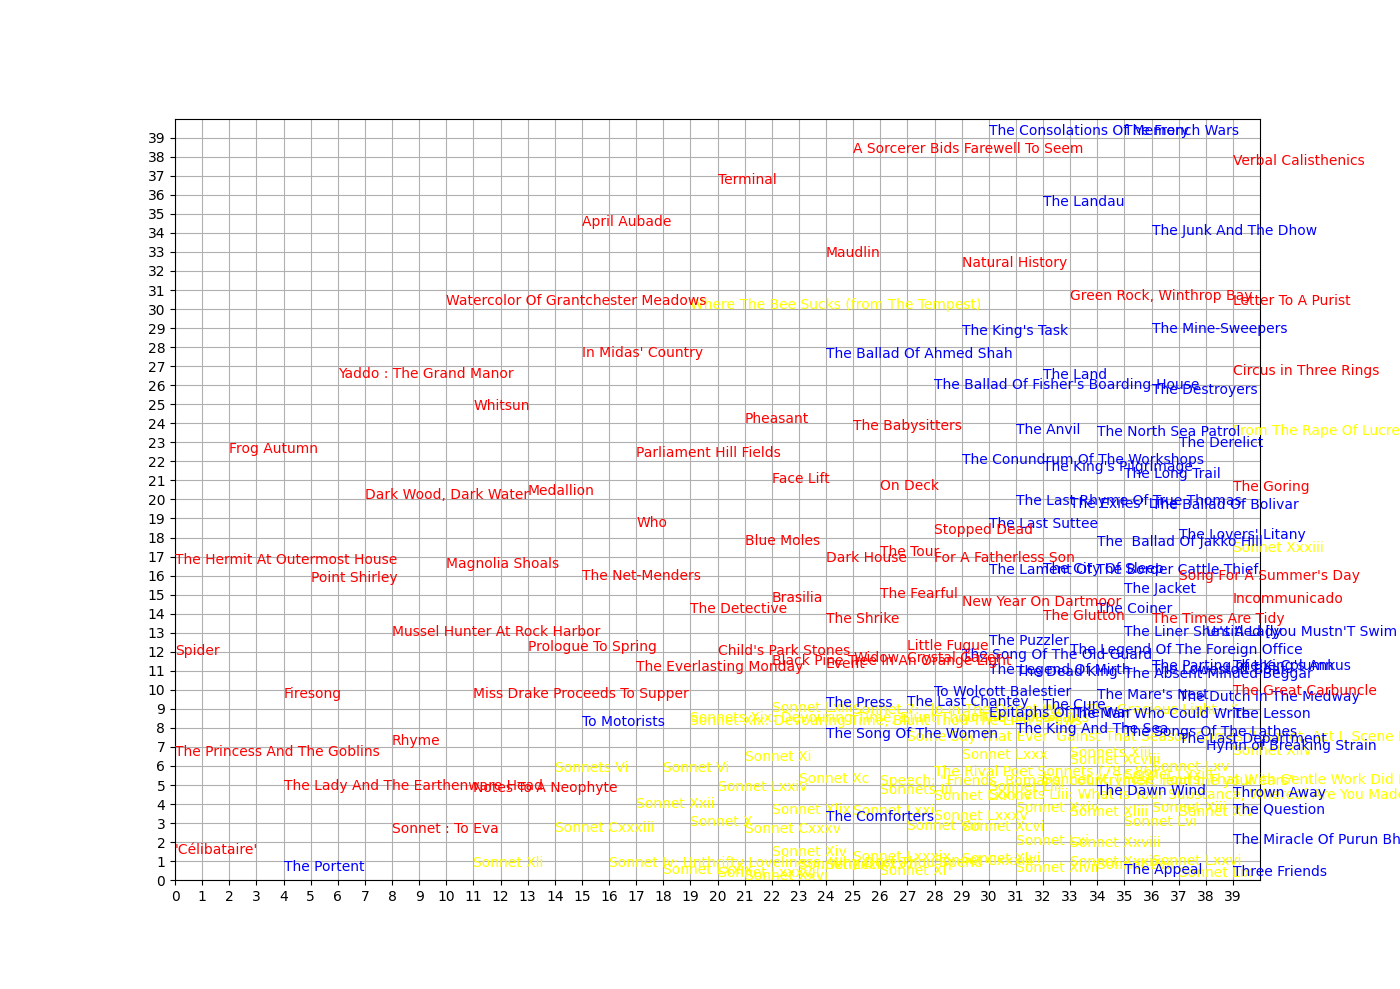
\includegraphics[scale=0.35]{Imagenes/WShakespeareRKiplingSPlathGlove300G40x40.png}
\end{center}
\section*{Conclusiones}
De los resultados de la experimentación pude encontrar datos muy interesantes incluído que tal parece que es más importante la nacionalidad a la cual hayan sido pertenecientes los Poetas que a la época en que vivieron, aunque claramente también la época es un factor importante, durante esa etapa del experimento no se obtuvieron tantos empates entre poetas como cuando todos son dela misma nacionalidad(Reino Unido), sin embargo en el experimento dónde cada uno de los poeta era de nacionalidad distinta podemos ver que la segmentación dentro de la malla es más clara.

\begin{thebibliography}{}
\bibitem{Analisis de Poemas}
\url{https://github.com/JustGlowing/minisom/blob/master/examples/PoemsAnalysis.ipynb}
\bibitem{Sitio para descargar los poemas}
\url{https://www.poemhunter.com/}
\bibitem{MiniSOM}
\url{https://pypi.org/project/MiniSom/#description}
\bibitem{Glove}
\url{https://en.wikipedia.org/wiki/GloVe_(machine_learning)}
\bibitem{SOM}
\url{https://en.wikipedia.org/wiki/Self-organizing_map}
\end{thebibliography}

\end{document}